\section{ATM}
\marginnote{From ./AE-Specifications-ETH/standalone/ATM.tex}

In the early 1990s, the \textsc{ATM Forum} became the battleground for a pivotal debate in networking: how to manage congestion in a cell-based fabric designed to unify voice, video, and data traffic. The two main contenders were \textbf{Hop-by-Hop Flow Control} and \textbf{Rate-Based Flow Control}. Each represented a fundamentally different view of how best to achieve performance guarantees and fairness across a heterogeneous, multi-hop network composed of 53-byte cells.

\subsection{The Challenge: ATM’s Dual Mandate}

ATM was envisioned as the unifying transport for all digital communication, requiring it to offer both the deterministic timing of circuit-switched networks and the efficiency of statistical multiplexing. This meant that congestion control was not merely a performance tweak, but a contractual necessity to maintain promised QoS levels.

ATM’s cut-through switching and small fixed-size cells eliminated much of the buffering flexibility available to IP networks. It had to prevent congestion, not recover from it.

\subsection{Hop-by-Hop Flow Control}

Hop-by-hop flow control works by applying \textit{local backpressure}: each switch monitors its output buffers and signals its upstream neighbor to slow or stop traffic as congestion builds.

\begin{marginfigure}
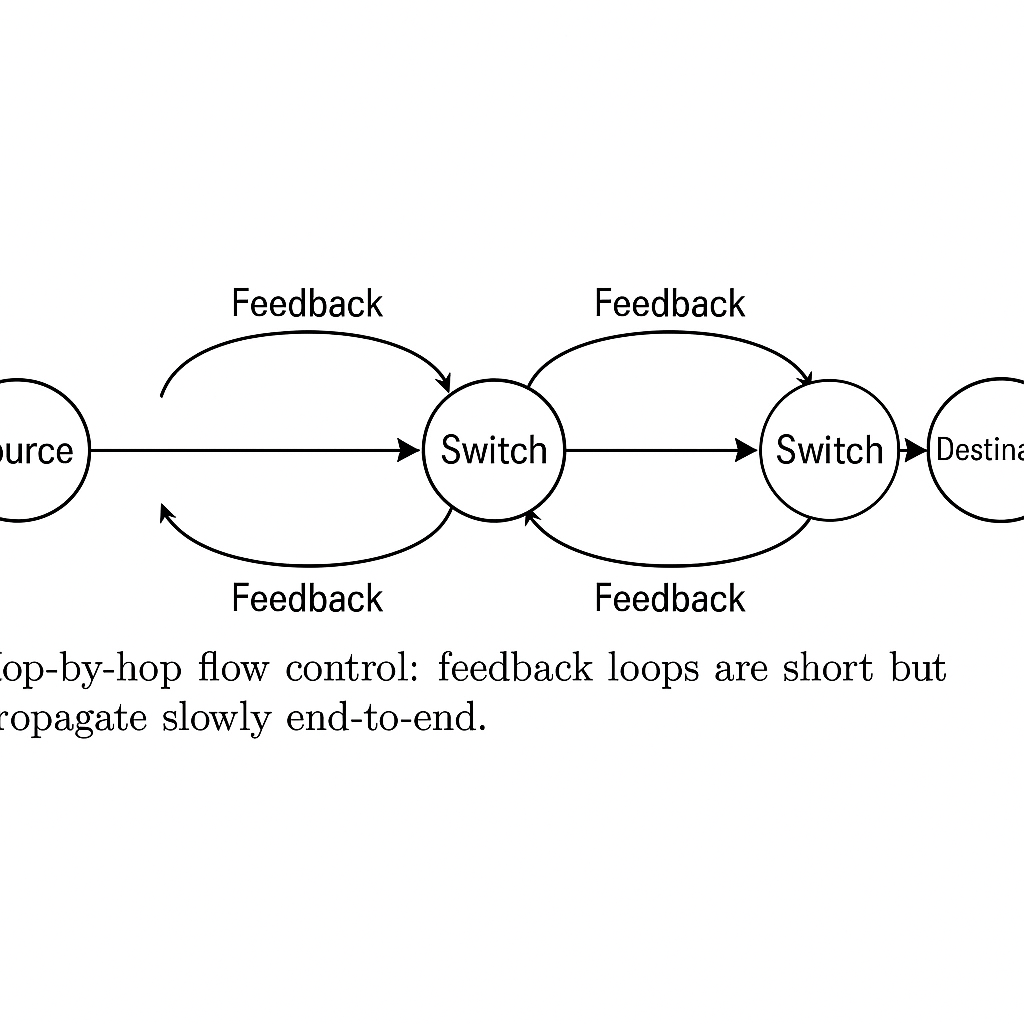
\includegraphics[width=\linewidth]{../../../FIGURES/ATM.png}
\caption{Hop-by-hop flow control: feedback loops are short but propagate slowly end-to-end.}
\end{marginfigure}

\paragraph{Advantages}
\begin{itemize}
  \item Immediate local reaction to congestion.
  \item Fine-grained control over buffer occupancy.
  \item Simple logic for small or low-diameter networks.
\end{itemize}

\paragraph{Drawbacks}
\begin{itemize}
  \item Scalability concerns: lacks consistent end-to-end semantics.
  \item Head-of-line blocking and poor latency propagation in long paths.
  \item Fragile under path diversity and route reconfiguration.
\end{itemize}

\subsection{Rate-Based Flow Control}

Rate-based flow control, standardized as part of the ATM \textsc{ABR (Available Bit Rate)} service class, aimed to regulate traffic from the \textit{edge}. Sources declare a desired transmission rate, and switches generate \textbf{Resource Management (RM)} cells containing congestion feedback. These RM cells traverse the path forward and backward, carrying fields such as \textit{Explicit Rate (ER)} that guide sender behavior.

\paragraph{Advantages}
\begin{itemize}
  \item End-to-end perspective scales better with network size.
  \item Enables policy-driven traffic contracts and rate shaping.
  \item Compatible with QoS-aware routing and admission control.
\end{itemize}

\paragraph{Drawbacks}
\begin{itemize}
  \item More complex per-switch logic and state maintenance.
  \item Relies on timely and reliable RM cell feedback.
  \item Convergence time can be slow in bursty or highly dynamic conditions.
\end{itemize}

\subsection{The Verdict: Standardization}

After extensive debate, the ATM Forum chose \textbf{Rate-Based Flow Control} as the official standard. This decision reflected a belief in the \textit{end-to-end model} of networking, better alignment with telco administration, and superior support for \textsc{SLAs} (Service Level Agreements). Switch vendors also favored rate-based schemes for their reduced buffer requirements and predictability.

\subsection{Legacy and Modern Echoes}

Although ATM faded from prominence, the ideas from its flow control debate echo through modern networking:

\begin{itemize}
  \item \textbf{InfiniBand} and \textbf{credit-based Ethernet} revived hop-by-hop flow control for low-latency datacenter fabrics.
  \item \textbf{TCP Vegas} and \textbf{XCP} extended the rate-based idea into congestion-aware transport.
  \item \textbf{PFC} and \textbf{QCN} in Data Center Bridging (DCB) illustrate hybrid approaches that combine both paradigms.
\end{itemize}

In hindsight, both models have value—hop-by-hop for tight fabrics with predictable topology; rate-based for scalable, heterogeneous systems. The ATM Forum chose well for its assumptions—but the future fragmented.

\subsection{Conclusion}

The ATM Forum's choice to standardize rate-based flow control was less a dismissal of hop-by-hop than a reflection of the broader ambitions of the ATM architecture. It aimed to build a global, carrier-grade network substrate. In contrast, datacenters—where predictability and tight control dominate—would later rediscover the strengths of localized flow control.

\begin{quote}
\itshape
Rate-based flow control won the standard. But hop-by-hop flow control won the datacenter.
\end{quote}
